 \chapter{ 'n Voorstelling van chemiese verandering}
\fancyfoot[LO,RE]{Chemie: Chemiese verandering}
   % \setcounter{figure}{1}
    %\setcounter{subfigure}{1}
    \label{337cc49099d6e82169c54b5d0fc3878f}
         \section{Introduction}
    \nopagebreak

Soos ons reeds genoem het, kan 'n aantal veranderinge plaasvind wanneer elemente met mekaar verbind. Hierdie veranderinge kan of \textsl{fisies} of \textsl{chemies} wees. In hierdie hoofstuk sal ons van naderby kyk na die chemiese veranderinge. Een wyse waarop chemiese veranderinge voorgestel kan word, is deur middel van \textbf{gebalanseerde chemiese vergelykings}. 'n Chemiese vergelyking beskryf 'n chemiese reaksie deur die gebruik van simbole vir die elemente wat betrokke is. As ons byvoorbeeld kyk na die reaksie tussen yster ($\text{Fe}$) en swawel ($\text{S}$) om ystersulfied ($\text{FeS}$) te vorm, kan ons hierdie veranderinge beskryf in 'n sinsnede of as 'n woordvergelyking of deur die gebruik van chemiese simbole:
%\begin{itemize}[noitemsep]
 \textbf{Sinsnede:} Yster reageer met swawel om ystersulfied te vorm.\\
 \textbf{Woordvergelyking:} Yster $+$ swawel $\to$ ystersulfied \\
 \textbf{Chemiese simbole:} $\text{Fe} + \text{S} \to \text{FeS}$\\

Nog 'n voorbeeld kan wees:
\textbf{Sinsnede:} Ammoniak reageer met suurstof om stikstofmonoksied en water te vorm.\\ 
\textbf{Woordvergelyking:} Ammoniak $+$ suurstof $\to$ stikstofmonoksied $+$ water\\
\textbf{Chemiese simbole:} $4{\text{NH}}_{3} + 5{\text{O}}_{2} \to 4\text{NO} + 6{\text{H}}_{2}\text{O}$\\
Verbindings aan die linkerkant van die pyltjie word die \textbf{reaktanse} genoem. Dit is wat nodig is vir die
reaksie om plaas te vind. Die verbindings aan die regterkant word die \textbf{produkte} genoem. Dit is die stowwe wat gevorm word uit die reaksie.\par 
Om 'n gebalanseerde chemiese vergelyking te kan neerskryf, is daar 'n aantal belangrike stappe
wat eers gevolg moet word: 
      \label{m38721*id62681}\begin{enumerate}[noitemsep, label=\textbf{\arabic*}. ] 
            \label{m38721*uid1}\item Maak seker jy ken die chemiese simbole vir die elemente wat betrokke is in die reaksie
\label{m38721*uid2}\item Jy moet in staat wees om die chemiese formules vir verskillende reaktanse en produkte neer te skryf
\label{m38721*uid3}\item Balanseer die chemiese vergelykings deur toepassing van die wette wat handel oor chemiese verandering 
\label{m38721*uid4}\item Maak seker jy ken die simbole wat die fases aandui in die vergelyking
\end{enumerate}
Ons sal na elk van hierdie stappe afsonderlik kyk in die volgende afdelings.
    \label{m38721*cid2}
            \subsection*{Chemiese simbole}
            \nopagebreak
Dit is baie belangrik om die chemiese simbole vir die algemene elemente in die Periodieke Tabel te ken
sodat jy in staat sal wees om chemiese vergelykings neer te skryf en verskillende verbindings uit te ken.\\
            \begin{activity}{Hersiening van algemene chemiese simbole}
            \nopagebreak
      \label{m38721*id62763}\begin{itemize}[noitemsep]
            \label{m38721*uid5}\item Skryf die chemiese simbole en name neer van al die elemente wat jy ken.
\label{m38721*uid6}\item Vergelyk jou lys met 'n ander leerder s’n en voeg enige simbole en name by wat by jou ontbreek.
\label{m38721*uid7}\item Maak seker jy ken die simbole van ten minste die eerste 36 elemente in die periodieke tabel. Jy moet ook die simbole leer ken van ander algemene elemente wat nie onder die eerste 36 is nie.
\label{m38721*uid8}\item Stel 'n kort toets op oor die benaming van elemente en verbindings vir iemand anders in die klas en ruil dan toetse met hulle sodat elkeen  'n kans kry om  'n toets te beantwoord.
\end{itemize}
\end{activity}
    \label{m38721*cid3}
\subsection*{Die skryf van chemiese formules}
\nopagebreak
\label{m38721*id62835} 'n \textbf{Chemiese formule} is 'n bondige manier waarop inligting oorgedra kan word oor die atome waaruit 'n bepaalde chemiese verbinding bestaan. 'n Chemiese formule toon elke element se simbool en wys ook hoeveel atome van elke element gevind word in die verbinding. Die aantal atome (indien meer as een) word as onderskrif aangedui.\par 
Die volgende oefening is vir hersiening. As jy nie kan onthou hoe om chemiese formules te skryf nie, gaan soek hulp in hoofstuk~\ref{chap:classification}.

\begin{exercises}{Revision of chemical formulae}
{
\begin{enumerate}[noitemsep, label=\textbf{\arabic*}.]
  \item Skryf die chemiese formule vir elk van die volgende verbindings neer:
\begin{enumerate}[noitemsep, label=\textbf{\alph*}. ]
 \item yster (III) chloried
\item sinknitraat
\item aluminiumsulfaat
\item kalsiumhidroksied
\item magnesiumkarbonaat
\item die produk wanneer koolstof met suurstof reageer
\item die produk wanneer waterstof reageer met stikstof
\item kaliumoksied
\item koper (II) bromied
\item kaliumdichromaat
\end{enumerate}
\item Skryf die naam vir elk van die volgende verbindings neer:
\begin{enumerate}[noitemsep, label=\textbf{\alph*}. ]
 \item $\text{SO}_2$
\item $\text{KMnO}_4$
\item $\text{(NH}_{4}\text{)}_{2}\text{SO}_{4}$
\item $\text{BaF}_2$
\item $\text{Cr(HSO}_{4}\text{)}_{3}$
\item $\text{CH}_{4}$
\end{enumerate}
\end{enumerate}

\insertpracticeinfo{2}
}
\end{exercises}

  \label{m38721**end}
         \section{Balansering van chemiese vergelykings}
    \nopagebreak


            \subsection*{Die wet van die behoud van massa}
            \nopagebreak
Ten einde 'n chemiese vergelyking te balanseer, is dit belangrik om die wet van die behoud van massa te verstaan.
\Definition{Die wet van die behoud van massa} {Die massa van 'n geslote sisteem van stowwe sal konstant bly, ongeag die prosesse wat binne die stelsel plaasvind. Materie kan verander van vorm, maar kan nie geskep of vernietig word nie. Vir enige chemiese proses in 'n geslote stelsel sal die massa van die reaktanse  gelyk wees aan die massa van die produkte. } 
In 'n chemiese vergelyking moet die \textbf{massa} van die reaktanse gelyk wees aan die massa van die produkte. Om seker te maak dat dit die geval is, moet die aantal \textbf{atome} van elke element in die reaktanse ooreenstem met die aantal atome van dieselfde elemente in die produkte.  'n Voorbeeld word hier aangetoon:
\begin{table}[H]
\begin{center}
\begin{tabular}{|p{3cm}p{3cm}|p{3cm}|}\hline
\scalebox{.4}{
\begin{pspicture}(0,0)(15,15)
\rput(0,0.5){\psframe(0,0)(3,2)
\rput(0.1,0){\multirput(0.2,0.2)(0.4,0){7}{\pscircle(0,0){0.2}}
\multirput(0.4,0.55)(0.4,0){6}{\pscircle(0,0){0.2}}
\multirput(0.2,0.9)(0.4,0){7}{\pscircle(0,0){0.2}}}}
\end{pspicture}} & 
\scalebox{.4}{
\begin{pspicture}(0,0)(15,15)
\rput(0,0.5){\psframe(0,0)(3,2)
\rput(0.1,0){\multirput(0.2,0.2)(0.4,0){7}{\pscircle[fillstyle=solid,fillcolor=gray](0,0){0.2}}
\multirput(0.4,0.55)(0.4,0){6}{\pscircle[fillstyle=solid,fillcolor=gray](0,0){0.2}}
\multirput(0.2,0.9)(0.4,0){7}{\pscircle[fillstyle=solid,fillcolor=gray](0,0){0.2}}}}
\end{pspicture}} & 
\scalebox{.4}{
\begin{pspicture}(0,0)(15,15)
\rput(0,0.5){\psframe(0,0)(3,2)
\rput(0.1,0){\multirput(0.2,0.2)(0.4,0){7}{\pscircle[fillstyle=solid,fillcolor=gray](0,0){0.2}}
\multirput(0.4,0.55)(0.4,0){6}{\pscircle(0,0){0.2}}
\multirput(0.2,0.9)(0.4,0){7}{\pscircle[fillstyle=solid,fillcolor=gray](0,0){0.2}}}}
\end{pspicture}}} \\ \hline
\multicolumn{3}{|c|}{$\text{Fe} + \text{S} \to \text{FeS}$} \\ \hline
Massa van een atoom van $\text{Fe}$ is $55,8$ & Massa van een atoom van $\text{S}$ is $32,1$ & Massa van een atoom van $\text{FeS}$ is $87,9$  \\ \hline
\multicolumn{2}{|c|}{Massa van reaktanse is $87,9$} & Massa van die produkte is $87,9$ \\ \hline
\end{tabular}
\end{center}
\label{tab:conservmass}
\end{table}
\Tip{Iron is a metal, when we represent it in a balanced chemical equation, we write only $\text{Fe}$. Sulphur occurs as $\text{S}_{8}$ but we write only the empirical formula: $\text{S}$. We do this for all network structures. Writing formulae like this represents \textsl{one unit} of the compound or network strucutre.}
Om die \textbf{massa van die molekule} te bereken gebruik ons die relatiewe atoommassas vir yster en swael, soos gesien in tabel~\ref{tab:conservmass}. Jy sal sien dat die massa van die reaktanse gelyk is aan die massa van die produkte.  'n Chemiese vergelyking wat \textbf{gebalanseerd} is, sal altyd gebaseer wees op die \textbf{wet van die behoud van massa} en die \textbf{wet van die behoud van atome}.  
      \label{m38726*eip-619}
            \begin{activity}{Balansering van chemiese vergelykings}
            \nopagebreak
\begin{enumerate}[noitemsep, label=\textbf{\arabic*}]
\item            \label{m38726*eip-695}Jy benodig: gekleurde balle (of albasters), wondergom, 'n vel papier en gekleurde penne.\\
Ons sal probeer om die volgende vergelyking te balanseer:
\label{m38726*eid0342}\nopagebreak\noindent{}
    \begin{equation*}
    \text{Al}+{\text{O}}_{2}\to {\text{Al}}_{2}{\text{O}}_{3}
      \end{equation*}
Neem 1 bal van 'n kleur. Dit verteenwoordig 'n molekule van $\text{Al}$. Neem twee balle van 'n ander kleur en plak hulle saam. Dit verteenwoordig 'n molekule van ${\text{O}}_{2}$. Plaas hierdie molekules aan jou linkerkant. Neem nou twee balle van een kleur en drie balle van 'n ander kleur om ${\text{Al}}_{2}{\text{O}}_{3}$ te vorm. Plaas hierdie verbinding aan jou regterkant. Teken gekleurde sirkels op 'n stuk papier om die balle te verteenwoordig. Trek 'n lyn in die middel van die papier om die verdeling van die molekules aan die linkerkant en aan die regterkant moontlik te maak.\\
Tel die aantal balle aan die linker- en regterkant. Is daar dieselfde hoeveelheid balle van elke kleur aan beide kante? As dit nie so is nie, is  die vergelyking nie gebalanseerd nie. Hoeveel balle sal jy moet toevoeg aan elke kant om te sorg dat daar ewe veel aan albei kante is? Hoe sal jy hierdie balle byvoeg?\\
Jy sal vind dat jy  4 balle nodig het van een kleur vir $\text{Al}$ en 3 pare balle van 'n ander kleur (d.w.s. 6 balle in totaal) vir die ${\text{O}}_{2}$ aan die linkerkant. Aan die regterkant sal jy  2 groepe van balle vir ${\text{Al}}_{2}{\text{O}}_{3}$. Ons s\^{e} dat die  gebalanseerde vergelyking as volg is:\\
    $4\text{Al}+3{\text{O}}_{2}\to 2{\text{Al}}_{2}{\text{O}}_{3}$

\item Gebruik jellietots en tandestokkies om die volgende chemiese vergelyking te bou. Maak seker die atome balanseer. Gebruik dieselfde kleur jellietots vir dieselfde atome.\\
$\text{C} + {\text{H}}_{2}\text{O} \to {\text{CO}}_{2} + {\text{CO}} + \text{H}_{2}$ \\
Voeg verbindings by totdat die atome gebalanseer is. Skryf die vergelyking neer en gebruik 'n ko\"{e}ffisient om aan te dui hoeveel verbindings jy gebruik, byvoorbeeld, as jy drie watermolekules moes gebruik, skryf dan $3{\text{H}}_{2}\text{O}$ 

\item Gebruik bal-en-stoktekeninge om die atome in die volgende reaksie te balanseer:\\
${\text{NH}}_{3} + {\text{O}}_{2} \to {\text{NO}} + \text{H}_{2}\text{O}$ \\
Gebruik jou tekeninge om 'n gebalanseerde chemiese vergelyking vir die reaksie neer te skryf.

\item Lood ($\text{Pb}$), lood (IV) oksied (${\text{PbO}}_{2}$) en swawelsuur  (${\text{H}}_{2}{\text{SO}}_{4}$) word gebruik in motorbatterye. Die volgende reaksie vind plaas:
$\text{Pb} + \text{PbO}_{2} + \text{H}_{2}\text{SO}_{4} \to {\text{PbSO}}_{4} + {\text{H}}_{2}\text{O}$ \\
Sny sirkels uit vier verskillende kleure papier om elkeen van die atome te verteenwoordig. Bou 'n paar van die verbindings met behulp van die gekleurde papier ($\text{Pb}$ $\text{PbO}_{2}$ $\text{H}_{2}\text{SO}_{4}$). Dit is die reaktanse. Moenie die produkte bou nie. Herrangskik die atome sodat die produkte gevorm word. Voeg meer reaktanse by as dit nodig is om die atome te balanseer. (Bv. jy sal twee $\text{H}_{2}\text{SO}_{4}$ molekules benodig). Gebruik wat jy geleer het om 'n gebalanseerde vergelyking neer te skryf vir die reaksie.
\end{enumerate}
 \begin{center}
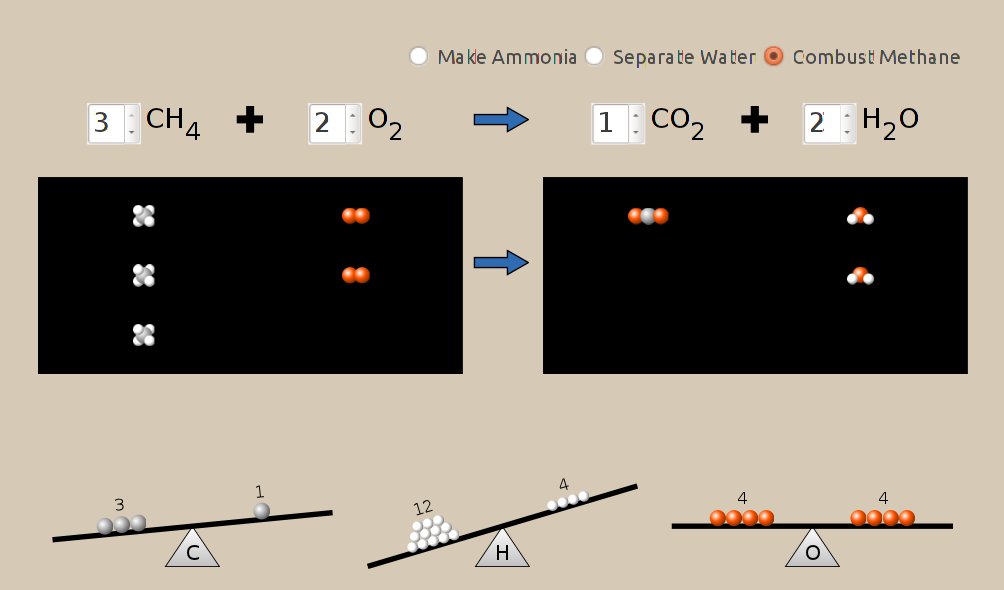
\includegraphics[width=.6\textwidth]{photos/BalancingChemEqu.png}\par
 \end{center}
\end{activity}
\par \label{m38726*uid10}
            \subsection*{Stappe om 'n chemiese vergelyking te balanseer deur middel van inspeksie}
            \nopagebreak
Wanneer jy 'n chemiese vergelyking wil balanseer, is daar 'n aantal stappe wat gevolg moet word.
        \label{m38726*id63712}\begin{enumerate}[noitemsep, label=\textbf{Stap \arabic*}:]
\item Identifiseer die reaktanse en die produkte in die reaksie en skryf hul chemiese formules neer.
\item Skryf die vergelyking deur die reaktanse aan die linkerkant van die pyl en die produkte aan die regterkant van die pyl te plaas.
\item Tel die aantal atome van elke element in die reaktanse en die aantal atome van elke element in die produkte.
\item Indien die vergelyking nie gebalanseer is nie, verander die koëffisiënte van die molekules totdat die aantal atome van elke element aan weerskante van die vergelyking balanseer.
\item Maak seker dat die atome werklik gebalanseerd is.
\item (ons sal later hierna kyk): Voeg enige ekstra besonderhede van die vergelyking by, bv. fase-simbole
\end{enumerate}
\par
            \label{m38726*secfhsst!!!underscore!!!id296}
      \noindent
\begin{wex}{Balansering van chemiese vergelykings I}{Balanseer die volgende vergelyking:
\begin{center}
${\text{Mg} + \text{HCl} \rightarrow \text{MgCl}_{2} + \text{H}_{2}}$\\
\end{center}
}
{
\westep{Omdat die vergelyking reeds vir jou neergeskryf is, kan jy direk voortgaan en begin om die aantal atome van elke element in die reaktanse en die produkte te tel.}

Reaktanse: $\text{Mg} = 1 ~\text{atoom;}~ \text{H} = 1 ~\text{atoom;}~ \text{Cl} = 1 ~\text{atoom}$

Produkte: $\text{Mg} = 1 ~\text{atoom;}~ \text{H} = 2 ~\text{atome;}~ \text{Cl} = 2 ~\text{atome}$
\westep{Balanseer die vergelyking}
Die vergelyking is nie gebalanseer nie aangesien daar 2 chlooratome in die produk en slegs 1 in die reaktanse teenwoordig is. As ons 'n koëffisiënt van 2 by die HCl voeg om die aantal H- en Cl-atome te verhoog by die reaktanse, sal die vergelyking soos volg lyk:
\begin{center}
${\text{Mg} + 2\text{HCl} \rightarrow \text{MgCl}_{2} + \text{H}_{2}}$\\
\end{center}


\westep{Maak seker dat die atome gebalanseer is }
As ons die atome aan elke kant van die vergelyking tel, vind ons die volgende:

Reaktanse: $\text{Mg} = 1;~ \text{H} = 2;~ \text{Cl} = 2$

Produkte: $\text{Mg} = 1;~ \text{H} = 2;~ \text{Cl} = 2$

Die vergelyking is nou gebalanseer. Die finale vergelyking is:
\begin{center}
${\text{Mg} + 2\text{HCl} \rightarrow \text{MgCl}_{2} + \text{H}_{2}}$
\end{center}
}
\end{wex}
    \noindent
\par
            \label{m38726*secfhsst!!!underscore!!!id394}
      \noindent
\begin{wex}{Balansering van chemiese vergelykings II}{Balanseer die volgende vergelyking:
\begin{center}
${\text{CH}_{4} + \text{O}_{2} \rightarrow \text{CO}_{2} + \text{H}_{2}\text{O}}$
\end{center}
}
{
\westep{Tel die aantal atome van elke element in die reaktanse en produkte}

Reaktanse: $\text{C} = 1;~ \text{H} = 4;~ \text{O} = 2$

Produkte: $\text{C} = 1;~ \text{H} = 2;~ \text{O} = 3$


\westep{Balanseer die vergelyking}
As ons 'n koëffisiënt van 2 by $\text{H}_{2}\text{O}$, voeg, dan is die aantal waterstofatome in die produkte gelyk aan  4, wat   dieselfde is  as vir die reaktanse. Die vergelyking sal die volgende wees:

\begin{center}
${\text{CH}_{4} + \text{O}_{2} \rightarrow \text{CO}_{2} + 2\text{H}_{2}\text{O}}$\\
\end{center}


\westep{Maak seker dat die atome balanseer}
Reaktanse: $\text{C} = 1;~ \text{H} = 4;~ \text{O} = 2$
Produkte: $\text{C} = 1;~ \text{H} = 4; ~\text{O} = 4$

Jy sal sien dat, hoewel die aantal waterstofatome nou balanseer, daar meer suurstof atome in die produkte is. Jy moet nou die vorige stap herhaal. As ons 'n koëffisiënt van 2 aan die voorkant van die $\text{O}_{2}$, plaas, sal ons die aantal suurstof atome verdubbel in die reaktanse. Die nuwe vergelyking is:
\begin{center}
${\text{CH}_{4} + 2\text{O}_{2} \rightarrow \text{CO}_{2} + 2\text{H}_{2}\text{O}}$
\end{center}
Wanneer ons die aantal atome weer kontroleer, vind ons dat die aantal atome van elke element in die reaktanse dieselfde is as die aantal in die produkte. Die vergelyking is nou gebalanseer.
}
\end{wex}
    \noindent
\label{m38726*secfhsst!!!underscore!!!id501}
      \noindent
\par
            \label{m38726*secfhsst!!!underscore!!!id590} 
      \noindent
\begin{wex}{Balansering van chemiese vergelykings III}{In ons liggame reageer suiker ${\text{(C}_{6}\text{H}_{12}\text{O}_{6}\text{)}}$ met suurstof wat ons inasem om koolstofdioksied, water en energie te produseer. Skryf die gebalanseerde vergelyking vir hierdie reaksie neer.}
{\westep{Identifiseer die reaktanse en produkte in die reaksie en skryf hul chemiese formules neer.}

Reaktanse: suiker (${\text{C}_{6}\text{H}_{12}\text{O}_{6}}$) en suurstof (${\text{O}_{2}}$)

Produkte: koolstofdioksied (${\text{CO}_{2}}$) en water (${\text{H}_{2}\text{O}}$)\\

\westep{Skryf die vergelyking neer deur die reaktanse aan die linkerkant van die pyl en die produkte aan die regterkant te plaas}
    $\text{C}_{6}\text{H}_{12}\text{O}_{6} + \text{O}_{2} \rightarrow \text{CO}_{2} + \text{H}_{2}\text{O}$

\westep{Tel die aantal atome van elke element in die reaktanse en die aantal atome van elke element in die produkte}
   Reaktanse: $\text{C} = 6;~ \text{H} = 12; ~\text{O} = 8$

   Produkte: $\text{C} = 1;~ \text{H} = 2; ~\text{O} = 3$

\westep{Verander die koeffisiënte van die molekules totdat die aantal atome van elke element aan beide kante van die vergelyking balanseer.}
Dit is makliker om te begin met koolstof omdat dit net een keer aan elke kant verskyn. As ons 'n $6$ aan die                                      voorkant van die ${\text{CO}_{2}}$, plaas, lyk die vergelyking soos volg:\\
    $\text{C}_{6}\text{H}_{12}\text{O}_{6} + \text{O}_{2} \rightarrow 6\text{CO}_{2} + \text{H}_{2}\text{O}$\\

   Reaktanse: $\text{C} = 6;~ \text{H} = 12; ~\text{O} = 8$

   Produkte: $\text{C} = 6;~ \text{H} = 2; ~\text{O} = 13$

\westep{Verander  weer die koëffisiënte om te probeer om die vergelyking te balanseer.}
Kom ons probeer om die aantal waterstofatome hierdie keer dieselfde te kry.\\
    $\text{C}_{6}\text{H}_{12}\text{O}_{6} + \text{O}_{2} \rightarrow 6\text{CO}_{2} + 6\text{H}_{2}\text{O}$

   Reaktanse: $\text{C} = 6;~ \text{H} = 12; ~\text{O} = 8$

   Produkte: $\text{C} = 6;~ \text{H} = 12; ~\text{O} = 18$

\westep{Nou het ons nog net nodig om die suurstofatome te balanseer.}
  $\text{C}_{6}\text{H}_{12}\text{O}_{6} + 6\text{O}_{2} \rightarrow 6\text{CO}_{2} + 6\text{H}_{2}\text{O}$

   Reaktanse: $\text{C} = 6;~ \text{H} = 12; ~\text{O} = 18$

   Produkte: $\text{C} = 6;~ \text{H} = 12; ~\text{O} = 18$
}
\end{wex}
    \noindent
% This simulation allows you to practice balancing simple equations.
%    \setcounter{subfigure}{0}
% 	\begin{figure}[H] % horizontal\label{m38806*transverse-waves}
%     \textnormal{Phet simulation for balancing equations}\vspace{.1in} \nopagebreak
%   \label{m38806*phet!!!underscore!!!sim}\label{m38806*phet-simulation}
%             \raisebox{-5 pt}{ 
\includegraphics[width=0.5cm]{col11305.imgs/summary_www.png}} { (Simulation:  lbD )}
%       \vspace{2pt}
%     \vspace{.1in}
%  \end{figure}       
%         \par \label{m38726*secfhsst!!!underscore!!!id763}

\begin{exercises}{Balancing simple chemical equations}
{
            \nopagebreak
Balanseer die volgende vergelykings:
\begin{enumerate}[noitemsep, label=\textbf{\arabic*}. ] 

\item  $\text{Mg} + {\text{O}}_{2} \to \text{MgO}$

\item ${\text{Ca}}+{\text{H}}_{2}\text{O} \to \text{Ca(OH)}_{2} + \text{H}_{2}$

\item ${\text{CuCO}}_{3} + {\text{H}}_{2}{\text{SO}}_{4} \to \text{CuSO}_{4} + {\text{H}}_{2}\text{O} + {\text{CO}}_{2}$

\item $\text{CaCl}_{2} + {\text{Na}}_{2}{\text{CO}}_{3} \to \text{CaCO}_{3} + {\text{NaCl}}$

\item ${\text{C}}_{12}{\text{H}}_{22}{\text{O}}_{11} + \text{O}_{2} \to \text{H}_{2}\text{O} + \text{CO}_{2}$

\item Bariumchloried reageer met swawelsuur om bariumsulfaat en soutsuur te vorm.

\item Etaan (${\text{C}}_{2}{\text{H}}_{6}$) reageer met suurstof om koolstofdioksied en stoom te vorm.

\item Ammoniumkarbonaat word dikwels gebruik as 'n vlugtige sout. Balanseer die volgende reaksie vir die ontbinding van ammoniumkarbonaat: ${\text{(NH}}_{4}{\text{)}}_{2}{\text{CO}}_{3} \text{(s)} \to {\text{NH}}_{3}\text{(aq)} + {\text{CO}}_{2} \text{(g)} + {\text{H}}_{2}\text{O} \ell}$

\item Waterstofbrandstofselle is uiters belangrik in die ontwikkeling van alternatiewe energiebronne. Baie van hierdie selle funksioneer deur die reaksie van waterstof- en suurstof- gasse om saam water te vorm;  'n reaksie wat ook elektrisiteit produseer. Balanseer die volgende vergelyking: ${\text{H}}_{2} \text{(g)} + {\text{O}}_{2} \text{(g)} \to {\text{H}}_{2} \text{O} \ell}$

\item Die sintese van ammoniak ($\text{NH}_{3}$), bekend gemaak deur die Duitse chemikus Fritz Haber in die vroe\"{e} 20ste eeu, is een van die belangrikste reaksies in die chemiese bedryf. Balanseer die volgende vergelyking vir die reaksie wat gebruik word om ammoniak te produseer:
${\text{N}}_{2} \text{(g)} + {\text{H}}_{2} \text{(g)} \to {\text{NH}}_{3} \text{(g)}$
\end{enumerate}

\practiceinfo
\begin{tabular}[h]{cccccc}
 (1.) lOW  &  (2.) lOZ   &  (3.) lOB  &  (4.) lOT  &  (5.) lOb  &  (6.) lOj  &  (7.) lOD  &  (8.) lOg  &  (9.) lO4  &  (10.) lO2  &
\end{tabular}
}
\end{exercises}

         \subsection*{Fase-simbole en ander inligting}
    \nopagebreak

Die fases van die verbindings kan uitgedruk word in  'n chemiese vergelyking. Dit word gedoen deur die korrekte simbool aan die regterkant van die formule te plaas. Die volgende vier simbole kan gebruik word: 
      \label{m38727*id65925}\begin{enumerate}[noitemsep, label=\textbf{\arabic*}. ] 
            \label{m38727*uid27}\item $\text{(g)}$ vir gasse
\label{m38727*uid28}\item $(\ell)$ vir vloeistowwe
\label{m38727*uid29}\item $\text{(s)}$ vir  vastestowwe
\label{m38727*uid30}\item $\text{(aq)}$ vir waterige oplossings 
\end{enumerate}
Om aan te toon dat hitte benodig word vir 'n reaksie, word 'n Griekse delta ($\Delta $) bo-op die pyltjie geplaas.
$\text{NH}_{4}\text{Cl} \xrightarrow{\Delta} \text{NH}_{3} + \text{HCl}$ \\

      \noindent
\begin{wex}{Balansering van chemiese vergelykings IV}{Soliede sinkmetaal reageer met  'n waterige soutsuuroplossing om 'n waterige oplossing van  sinkchloried ($\text{ZnCl}_{2}$) en waterstofgas te vorm. Skryf 'n gebalanseerde vergelyking vir hierdie reaksie neer.}{
\westep{Identifiseer die reaktanse en produkte en hul chemiese formules}
Die reaktanse is sink ($\text{Zn}$) en soutsuur ($\text{HCl}$). Die produkte is sink chloried ($\text{ZnCl}_{2}$) en waterstof ($\text{H}_{2}$).\\


\westep{Plaas die reaktanse aan die linkerkant van die vergelyking en die produkte aan die regterkant van die pyltjie.}
${\text{Zn} + \text{HCl} \rightarrow \text{ZnCl}_{2} + \text{H}_{2}}$


\westep{Balanseer die vergelyking}
Jy sal oplet dat die sinkatome balanseer, maar die chloor-en waterstofatome nie. Aangesien daar twee chlooratome aan die regterkant en slegs een aan die linkerkant is, sal ons by HCl 'n ko\"{e}ffisiënt van 2 plaas sodat daar twee chlooratome aan elke kant van die  vergelyking is.
${\text{Zn} + 2\text{HCl} \rightarrow \text{ZnCl}_{2} + \text{H}_{2}}$


\westep{Maak seker dat al die atome balanseer}
 As jy weer na die vergelyking kyk, sal jy sien dat al die atome nou gebalanseer is.


\westep{Maak seker dat alle inligting (bv. fase-simbole) bygevoeg is}
In die aanvanklike beskrywing is daar genoem dat sink 'n metaal is, dat soutsuur en sinkchloried beide waterige oplossings is  en dat waterstof 'n gas is.
$\text{Zn (s)} + \text{HCl (aq)} \rightarrow \text{ZnCl}_{2} \text{(aq)} + \text{H}_{2} \text{(g)}$
}
\end{wex}
    \noindent
\par

% \label{m38727*eip-44}The following video explains some of the concepts of balancing chemical equations.\newline
%     \setcounter{subfigure}{0}
% 	\begin{figure}[H] % horizontal\label{m38727*balancing-equations}
%     \textnormal{Khan Academy video on balancing chemical equations}\vspace{.1in} \nopagebreak
%   \label{m38727*yt-media1}\label{m38727*yt-video1}
%             \raisebox{-5 pt}{ 
\includegraphics[width=0.5cm]{col11305.imgs/summary_www.png}} { (Video:  P10062 )}
%       \vspace{2pt}
%     \vspace{.1in}
%  \end{figure}       \par \label{m38727*secfhsst!!!underscore!!!id1261}

\mindsetvid{Khan academy video on balancing equations}{VPemn}

 \begin{activity}{Fase-simbole}
            \nopagebreak
Skryf gebalanseerde vergelykings vir elk van die volgende reaksies, insluitend fase-simbole::\par 
      \label{m38727*id66796}\begin{enumerate}[noitemsep, label=\textbf{\arabic*}. ] 
        \label{m38727*uid33}\item Lood (II) nitraatoplossing reageer met 'n kaliumjodied oplossing om  'n neerslag van loodjodied te vorm, terwyl kaliumnitraat in oplossing bly.
\label{m38727*uid34}\item Wanneer aluminium metaal verhit word, reageer dit met soliede koperoksied om kopermetaal en  aluminiumoksied (${\text{Al}}_{2}{\text{O}}_{3}$) te produseer.
\label{m38727*uid35}\item Wanneer kalsiumchloried oplossing gemeng word met  'n silwernitraat oplossing, verskyn 'n wit neerslag (vaste stof) van silwerchloried. Kalsiumnitraat ($\text{{Ca(NO}}_{3}\text{)}}_{2}$) word ook in die oplossing gevorm.
\item Vaste ammonium karbonaat ontbind om drie gasprodukte te vorm.
        \end{enumerate}
\end{activity}
\begin{g_experiment}{Die verhouding tussen produkte en die reaktanse}
\textbf{Doel:} Om ondersoek in te stel na die verhouding tussen die hoeveelhede van die produkte en die reaktanse.\\
\textbf{Apparaat:}\\
\begin{minipage}{.5\textwidth}
 \begin{itemize}[noitemsep]
  \item fles
\item maatsilinder
\item waterbak
\item afleibuis
\item tregter met afsluitkraan
\item prop
\item natriumwaterstofkarbonaat ($\text{NaHCO}_{3}$) poeier
\item verdunde swawelsuur ($\text{H}_{2}\text{SO}_{4}$)
 \end{itemize}
\end{minipage}
\begin{minipage}{.5\textwidth}
\begin{center}
\scalebox{0.8}{
 \begin{pspicture}(0,0)(5,5)
\psset{unit=0.5cm,glassType=erlen}
\newpsstyle{white} {linestyle=solid,linecolor=black,linewidth=.1,fillstyle=solid,fillcolor=white}
 \pstChauffageBallon[recuperationGaz,doubletube,aspectLiquide1=white,niveauLiquide1=20]
\end{pspicture}
}
\end{center}
\end{minipage} \\
\textbf{Metode:} 
\begin{enumerate}[noitemsep,label=\textbf{\arabic*}]
 \item Weeg $20~\text{g}$ van $\text{NaHCO}_{3}$ af en plaas dit in 'n fles.
\item Stel die bogenoemde apparaat op.
\item Meet $5~\text{ml}$ van $\text{H}_{2}\text{SO}_{4}$ en gooi dit versigtig in die tregter.
\item Voeg die $\text{H}_{2}\text{SO}_{4}$ stadig by die $\text{NaHCO}_{3}$.
\item Neem waar wat gebeur.
\item Teken die volume van die gas aan wat in die maatsilinder versamel.
\item Herhaal die bogenoemde stappe, maar gebruik hierdie keer $10~\text{ml}$ van die $\text{H}_{2}\text{SO}_{4}$.
\item Skryf 'n gebalanseerde vergelyking vir hierdie reaksie neer. (Wenk: koolstofdioksied gas is gevorm, asook water en natriumsulfaat.)
\end{enumerate}
\textbf{Results and discussion:}\\
Jy moet daarop let dat meer gas gevorm word wanneer  'n groter hoeveelheid $\text{H}_{2}\text{SO}_{4}$ gebruik word. 
\end{g_experiment}

Gebalanseerde vergelykings is baie belangrik in chemie. Deur te werk met gebalanseerde vergelykings kan chemici  verskillende berekenings uitvoer en sodoende bepaal hoeveel van  'n sekere stof deelneem aan  'n reaksie. In 'n latere hoofstuk sal ons uitvind hoe om hierdie berekenings te maak. Ons kan gebalanseerde chemiese reaksies interpreteer in terme van die behoud van materie, die behoud van massa en die behoud van energie.
%     \setcounter{subfigure}{0}
% 	\begin{figure}[H] % horizontal\label{m38727*slidesharefigure}
%     \label{m38727*slidesharemedia}\label{m38727*slideshareflash}\raisebox{-5 pt}{ 
\includegraphics[width=0.5cm]{col11305.imgs/summary_www.png}} { (Presentation:  P10063 )} \end{figure}

\summary{VPeca}
            \nopagebreak
      \label{m38727*id67171}\begin{itemize}[noitemsep]
            \label{m38727*uid36}\item 'n \textbf{Chemiese vergelyking} gebruik simbole om 'n chemiese reaksie te beskryf.
\label{m38727*uid37}\item In 'n chemiese vergelyking, word \textbf{reaktanse} aan die linkerkant van die vergelyking geskryf en \textbf{produkte} aan die regterkant. Die pyltjie word gebruik om die rigting van die reaksie aan te toon.
\label{m38727*uid38}\item Wanneer  'n chemiese verandering voorgestel word, is dit belangrik om in staat te wees om die \textbf{chemiese formule} van  'n verbinding neer te skryf.
\label{m38727*uid39}\item In enige chemiese reaksie is die \textbf{wet van die behoud van massa} altyd van toepassing. Dit beteken dat die totale atoommassa van die reaktanse moet ooreenstem met die totale atoommassa van die produkte. Dit beteken ook dat die totale aantal atome van die reaktanse dieselfde moet wees as die totale aantal atome van die produkte.
\label{m38727*uid41}\item Indien die aantal atome van elke element in die reaktanse ooreenstem met die aantal atome van elke element in die produkte, is die vergelyking gebalanseer.
\label{m38727*uid42}\item Indien die getal atome van elke element in die reaktanse nie dieselfde is as die aantal atome van elke element in die produkte nie, is die vergelyking nie gebalanseer nie.
\item Ten einde 'n vergelyking te balanseer,  kan koëffisiënte geplaas word aan die voorkant van die reaktanse en die  produkte totdat die aantal atome van elke element dieselfde is aan beide kante van die vergelyking.
\end{itemize}


\begin{eocexercises}{Representing chemical change}
            \nopagebreak
\begin{enumerate}[noitemsep, label=\textbf{\arabic*}. ] 

\item Propaan is 'n brandstof wat algemeen gebruik word as 'n bron van hitte vir enjins en huise. Balanseer die volgende vergelyking vir die ontbranding van propaan:
${\text{C}}_{3}{\text{H}}_{8} \ell} + \text{O}_{2} \text{(g)} \to \text{CO}_{2} \text{(g)} + \text{H}_{2}\text{O} \ell}$

\item Metaan ($\text{CH}_{4}$) brand in suurstof volgens die volgende reaksie. \\
\begin{figure}[H]
\begin{center}
 \includegraphics[width=.8\textwidth]{photos/methane_O2_rxn.png}
\end{center}
\end{figure}

\begin{enumerate}[noitemsep, label=\textbf{\alph*}.]
 \item Teken bal-en-stokmodelle van die produkte om die diagramme te voltooi.
\item Skryf 'n gebalanseerde chemiese vergelyking vir die reaksie, insluitend fase-simbole.
\end{enumerate}

\item Chemiese wapens is in 1925 deur die Geneefse Protokol (konvensie) verbied. Volgens hierdie protokol mag geen chemikalieë wat giftige of versmorende gasse vrylaat, gebruik word as wapens nie. Wit fosfor, 'n baie reaktiewe allotroop van fosfor, is onlangs tydens 'n milit\^{e}re aanval gebruik. Fosfor brand kragtig in suurstof. Baie mense het ernstige brandwonde opgedoen en 'n paar het as gevolg daarvan gesterf. Die vergelyking vir hierdie spontane reaksie is:
        ${\text{P}}_{4}\left(\text{s}\right)+{\text{O}}_{2}\left(\text{g}\right)\to {\text{P}}_{2}{\text{O}}_{5}\left(\text{s}\right)$

    \begin{enumerate}[noitemsep, label=\textbf{\alph*}. ] 
    \item Balanseer die chemiese vergelyking.
    \item Bewys dat die wet van die behoud van massa gehoorsaam word tydens hierdie chemiese reaksie.
    \item Noem die produk wat tydens hierdie reaksie gevorm word.
    \item Klassifiseer die reaksie as endotermies of eksotermies. Gee 'n rede vir jou antwoord.
    \item Klassifiseer die reaksie as 'n sintese- of ontbindingsreaksie. Gee 'n rede vir jou antwoord.
    \end{enumerate}

% (DoE Exemplar Paper 2 2007)
\item Die volgende diagramme verteenwoordig die verbranding van etaan ($\text{C}_\text{H}_6$). Voltooi die diagramme en skryf 'n gebalanseerde vergelyking vir die reaksie neer. Dui die fase-simbole aan. \\

\scalebox{0.8} % Change this value to rescale the drawing.
{
\begin{pspicture}(0,-2.015)(10.04,2.015)
\definecolor{color6b}{rgb}{0.5882352941176471,0.5882352941176471,0.5882352941176471}
\definecolor{color7b}{rgb}{0.19607843137254902,0.19607843137254902,0.19607843137254902}
\psframe[linewidth=0.04,dimen=outer](3.98,2.005)(0.0,-1.975)
\psframe[linewidth=0.04,dimen=outer](10.04,2.015)(6.01,-2.015)
\rput{-32.038597}(0.25529027,1.656808){\pscircle[linewidth=0.04,linecolor=color6b,dimen=outer,fillstyle=solid,fillcolor=color6b](3.012965,0.3838178){0.24}}
\rput{-32.038597}(0.44232956,1.8115258){\pscircle[linewidth=0.04,linecolor=color6b,dimen=outer,fillstyle=solid,fillcolor=color6b](3.3759246,0.13544907){0.24}}
\pscircle[linewidth=0.04,linecolor=color7b,dimen=outer,fillstyle=solid,fillcolor=color7b](2.87,-0.735){0.24}
\pscircle[linewidth=0.04,dimen=outer](2.85,-0.385){0.12}
\pscircle[linewidth=0.04,linecolor=color7b,dimen=outer,fillstyle=solid,fillcolor=color7b](3.33,-0.735){0.24}
\pscircle[linewidth=0.04,dimen=outer](2.53,-0.745){0.12}
\pscircle[linewidth=0.04,dimen=outer](2.85,-1.085){0.12}
\pscircle[linewidth=0.04,dimen=outer](3.35,-1.085){0.12}
\pscircle[linewidth=0.04,dimen=outer](3.67,-0.745){0.12}
\pscircle[linewidth=0.04,dimen=outer](3.33,-0.385){0.12}
\pscircle[linewidth=0.04,linecolor=color6b,dimen=outer,fillstyle=solid,fillcolor=color6b](2.82,1.265){0.24}
\pscircle[linewidth=0.04,linecolor=color6b,dimen=outer,fillstyle=solid,fillcolor=color6b](3.26,1.265){0.24}
\rput{32.43465}(-0.57426614,-0.9315801){\pscircle[linewidth=0.04,linecolor=color6b,dimen=outer,fillstyle=solid,fillcolor=color6b](1.3143191,-1.4529942){0.24}}
\rput{32.43465}(-0.38976568,-1.0939419){\pscircle[linewidth=0.04,linecolor=color6b,dimen=outer,fillstyle=solid,fillcolor=color6b](1.6856809,-1.2170057){0.24}}
\rput{-95.96166}(2.008164,2.2169962){\pscircle[linewidth=0.04,linecolor=color6b,dimen=outer,fillstyle=solid,fillcolor=color6b](2.0028498,0.20381016){0.24}}
\rput{-95.96166}(2.3929713,1.6884707){\pscircle[linewidth=0.04,linecolor=color6b,dimen=outer,fillstyle=solid,fillcolor=color6b](1.9571501,-0.23381016){0.24}}
\pscircle[linewidth=0.04,linecolor=color6b,dimen=outer,fillstyle=solid,fillcolor=color6b](2.4,-1.615){0.24}
\pscircle[linewidth=0.04,linecolor=color6b,dimen=outer,fillstyle=solid,fillcolor=color6b](2.84,-1.615){0.24}
\pscircle[linewidth=0.04,linecolor=color6b,dimen=outer,fillstyle=solid,fillcolor=color6b](0.64,0.225){0.24}
\pscircle[linewidth=0.04,linecolor=color6b,dimen=outer,fillstyle=solid,fillcolor=color6b](1.08,0.225){0.24}
\rput{158.27188}(1.526796,-1.8859106){\pscircle[linewidth=0.04,linecolor=color6b,dimen=outer,fillstyle=solid,fillcolor=color6b](0.9443692,-0.7964446){0.24}}
\rput{158.27188}(0.7986616,-1.4203893){\pscircle[linewidth=0.04,linecolor=color6b,dimen=outer,fillstyle=solid,fillcolor=color6b](0.53563076,-0.6335554){0.24}}
\pscircle[linewidth=0.04,linecolor=color7b,dimen=outer,fillstyle=solid,fillcolor=color7b](0.81,1.325){0.24}
\pscircle[linewidth=0.04,dimen=outer](0.79,1.675){0.12}
\pscircle[linewidth=0.04,linecolor=color7b,dimen=outer,fillstyle=solid,fillcolor=color7b](1.27,1.325){0.24}
\pscircle[linewidth=0.04,dimen=outer](0.47,1.315){0.12}
\pscircle[linewidth=0.04,dimen=outer](0.79,0.975){0.12}
\pscircle[linewidth=0.04,dimen=outer](1.29,0.975){0.12}
\pscircle[linewidth=0.04,dimen=outer](1.61,1.315){0.12}
\pscircle[linewidth=0.04,dimen=outer](1.27,1.675){0.12}
\psline[linewidth=0.04cm,arrowsize=0.05291667cm 3.0,arrowlength=1.4,arrowinset=0.0]{->}(4.18,0.045)(5.64,0.025)
\end{pspicture} 
}

\item Balanseer die volgende chemiese vergelyking:
${\text{N}}_{2}{\text{O}}_{5}\to {\text{NO}}_{2}+{\text{O}}_{2}$ Teken submikroskopiese diagramme om hierdie reaksie te verteenwoordig.

\item Swawel kan geproduseer word deur die Clausproses. Hierdie proses vind in twee stappe plaas. Eers reageer waterstofsulfied met suurstof en dan word swaweldioksied toegelaat om te reageer met nog meer van die waterstofsulfied. Die vergelykings vir hierdie twee  reaksies:
\nopagebreak\noindent{}
    \begin{equation}
    \begin{array}{c}{\text{H}}_{2}\text{S}+{\text{O}}_{2}\to {\text{SO}}_{2}+{\text{H}}_{2}\text{O}\\ {\text{H}}_{2}\text{S}+{\text{SO}}_{2}\to \text{S}+{\text{H}}_{2}\text{O}\end{array}
      \end{equation}
Balanseer hierdie twee vergelykings.

\item Aspartaam, 'n kunsmatige versoeter, het die formule ${\text{C}}_{14}{\text{H}}_{18}{\text{N}}_{2}{\text{O}}_{2}$. Skryf die gebalanseerde vergelyking neer vir die verbranding (reaksie met die ${\text{O}}_{2}$) hiervan om ${\text{CO}}_{2}$ gas, vloeibare water $\text{H}_{2}\text{O}$, en ${\text{N}}_{2}$ gas te vorm. 
\end{enumerate}

\practiceinfo
\begin{tabular}[h]{cccccc}
 (1.) lOk  &  (2.) lO0  &  (3.) lO8  &  (4.) lO9  &  (5.) l2S  &  (6.) l2h  &  (7.) lTq  &
\end{tabular}
\end{eocexercises}
